\documentclass[10pt, a4paper]{article}

\usepackage[
  left=1cm, right=9cm,
  marginparwidth=6.8cm, marginparsep=1.2cm,
  top=1.2cm, bottom=1.2cm
]{geometry}

\usepackage[T1]{fontenc}
\usepackage[osf, sc]{mathpazo}
\usepackage[newcommands]{ragged2e}
\usepackage[final, tracking=true, kerning=true, spacing=true]{microtype}
\usepackage{textcomp}
\usepackage{graphicx}
\usepackage{pgfornament}
\usepackage[hidelinks, breaklinks=true]{hyperref}

\hypersetup{
  pdftitle={CV - David Álvarez Rosa},
  pdfauthor={David Álvarez Rosa}
}

\pagestyle{empty}
\setlength{\parindent}{0pt}
\AtBeginDocument{\RaggedRight}

\newcommand{\headingrule}[2]{%
  {#1\scshape\MakeLowercase{#2}\\[-0.7ex]}%
  \rule{\linewidth}{0.5pt}\par\vspace{2pt}%
}
\newcommand{\cvsection}[1]{\vspace{12pt}\headingrule{\large}{#1}}
\newcommand{\sideheading}[1]{\addvspace{10pt}\headingrule{\normalsize}{#1}}

\newcommand{\lineitem}[2]{%
  #1---#2\par\addvspace{4pt}%
}
\newcommand{\entry}[2]{%
  \textit{#1}\par{\small #2}\par\addvspace{8pt}%
}

\newcommand{\role}[4]{%
  {\bfseries #1}\hfill{\small #2}\par
  {\small #3}\par\smallskip
  #4\par\addvspace{9pt}%
}
\newcommand{\degree}[3]{%
  {\bfseries #1}\hfill{\small #2}\par\smallskip
  #3\par\addvspace{9pt}%
}

\begin{document}

\marginpar{\raggedright
  \vspace*{11pt}%
  {\centering
    \begin{tikzpicture}
      \node[inner sep=0pt] (p) {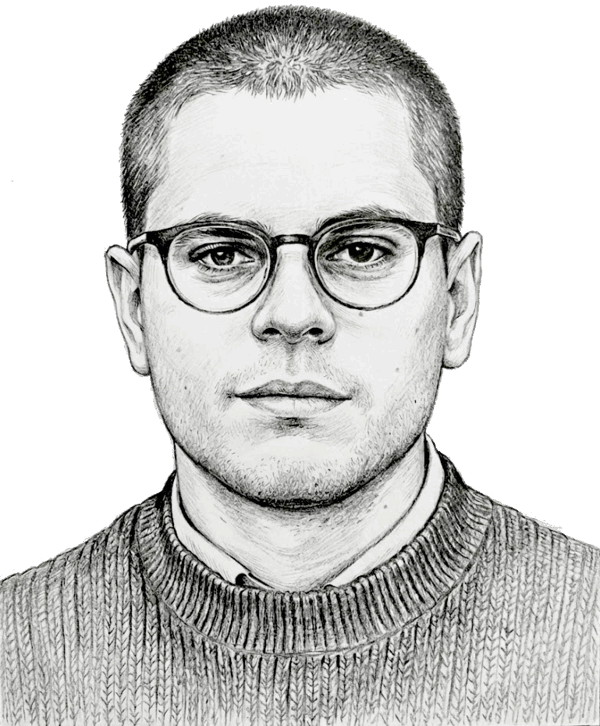
\includegraphics[width=0.50\linewidth]{portrait.png}};
      \node[anchor=south, yshift=2pt, inner xsep=2pt, inner ysep=1pt,
            fill=white, fill opacity=0.7, text opacity=1,
            font=\footnotesize\itshape] at (p.south) {That's me! March~2022.};
    \end{tikzpicture}\par}%
  \sideheading{Certifications}
  \lineitem{Advanced English (C1)}{Cambridge}
  \lineitem{Machine Learning}{Stanford University}
  \lineitem{Deep Learning}{deeplearning.ai}
  \lineitem{Blockchain}{Hong Kong University}
  \lineitem{Nova Talent Member}{Nova}

  \sideheading{Volunteering}
  \entry{Mathematics Tutor}{Training for the Mathematical Olympiads.}
  \entry{Volunteer @ Banco de Alimentos}{Food collection for people in need.}

  \sideheading{Honors \& Awards}
  \entry{Mathematical Olympiad}{Silver (local), honors (national).}
  \entry{Physics Olympiad}{Gold (local), silver (national).}
  \entry{Mobility Scholarship}{Research thesis at Toronto (\texteuro{}6k).}
  \entry{Tuition and Housing Scholarship}{University tuition and housing (\texteuro{}19k).}
  \entry{General Scholarship}{Full tuition plus annual stipend (\texteuro{}11k).}

  \sideheading{Languages}
  \lineitem{English}{Proficient}
  \lineitem{Spanish}{Native}
  \lineitem{Catalan}{Intermediate}

  \sideheading{Contact}
  \lineitem{Website}{\href{https://david.alvarezrosa.com}{david.alvarezrosa.com}}
  \lineitem{Email}{\href{mailto:david@alvarezrosa.com}{david@alvarezrosa.com}}
  \lineitem{LinkedIn}{\href{https://www.linkedin.com/in/david-alvarez-rosa/}{david-alvarez-rosa}}
  \lineitem{GitHub}{\href{https://github.com/david-alvarez-rosa}{david-alvarez-rosa}}
  \lineitem{Phone}{\href{tel:+34647133930}{+34\,647\,133\,930}}

  \par\vspace{22pt}\makebox[\linewidth][c]{\pgfornament[width=2.4cm]{156}}%
}


{\large\itshape Curriculum Vitae}\\[-1.2ex]%
\rule{\linewidth}{0.6pt}\par%
\vspace{1pt}%
{\huge\textbf{\href{https://david.alvarezrosa.com}{DAVID ÁLVAREZ ROSA}}\par}%
\vspace{10pt}%
{Mathematician and engineer based in sunny Dublin, passionate about
  low-latency, high-performance systems.\par}%
\vspace{6pt}%
{Currently working in algorithmic trading at Susquehanna; previously at
  Amazon, Sopra Steria, and Deloitte.\par}%
\vspace{6pt}%
{Holds a BSc in Mathematics, a BEng in Industrial Engineering, and an
  MSc in Artificial Intelligence.\par}%
\vspace{6pt}%

\cvsection{Experience}

\role{Software Engineer}{Jul 2024--Present}{Susquehanna International
  Group · Dublin, Ireland}{%
  High-frequency options trading. Low-latency market data and trading
  signals.  Mentor and interviewer.}

\role{Software Engineer II}{Mar 2022--Aug 2024}{Amazon · Madrid,
  Spain}{%
  Designed systems for 10M+ monthly active customers. Contributed to
  100+ internal repos. Won org hackathon. Promoted in 18 months (top
  5\%). Mentored 3. On-call.  Interviewer.}

\role{Machine Learning Engineer}{Apr 2024--Jul 2024}{Sopra Steria ·
  Remote}{%
  Researched, designed, and built a semantic cache for LLMs.}

\role{Risk Analyst}{Sep 2021--Mar 2022}{Deloitte · Madrid, Spain}{%
  Quantitative analysis of technological and cybersecurity risks for
  top-tier banking companies.}

\role{Visiting Researcher}{Sep 2020--Jun 2021}{Vector Institute ·
  Toronto, Canada}{%
  Research thesis on multimodal learning
  (\href{https://recomprehension.com}{recomprehension.com}).}

\role{Machine Learning Engineer}{Sep 2019--Feb 2020}{BCN eMotorsport ·
  Barcelona, Spain}{%
  Perception at Driverless UPC.  Served as LiDAR lead and collaborated
  on computer vision for a fully autonomous car.}

\cvsection{Education}

\degree{MSc in Artificial Intelligence}{9.00/10}{%
  Official study program focused on AI research and enabling PhD.
  Honors in 6 subjects.}

\degree{MSc in Mathematics}{}{%
  Math-lover part-time student. Dropout (joined Amazon).}

\degree{Research Thesis}{10/10 (A+)}{%
  Research thesis on multimodal learning at University of Toronto.}

\degree{BSc in Mathematics}{8.12/10 (top 10\%)}{%
  Rigorous and proof-oriented degree with a robust mathematical base.
  Honors in 9 subjects.}

\degree{BEng in Industrial Engineering}{8.03/10 (top 2\%)}{%
  Multidisciplinary and integrative vision of industrial engineering.
  Honors in 14 subjects.}

\end{document}
